\section{Hypothesis testing}

\subsection{Basic elements}
% critical fun., size, power, power function (\beta(\theta) = E_\theta[\phi(X)] is size at \theta \in \Theta_0 and power at \theta \in \Theta_1).
% goal is to max power controling size

\subsection{Testing simple hypotheses}
% LR Theorem, how to compute \gamma

\subsection{Testing composite hypotheses}

\subsection{Bayesian hypothses testing}

% Bayes factor
% p(H0|X) = rB / (1+rB) as a useful conversion between the two

Note that $B$ is defined only when proper priors are used for $\theta$. It is not well defined under improper priors.
Moreover, $B$ may be sensitive to the choice of prior distribution and/or the choice of prior hyperparameters.

\textbf{Remark: Connection between Bayes factor and LRT.}
\begin{itemize}
    \item The Bayes factor as the Bayesian analogue of LRT. We integrate over the parameter space $\theta_0$, not maximize over it. 
    The Bayes factor $B=\frac{p(x|\theta_0)}{p(x|\theta_1)}$ reduces to the NP test in the simple versus simple case.
    \item The Bayes factor can easily accommodate complicated composite hypotheses of any form, by integrating over $\Theta_0$ and $\Theta_1$ as in \blue{eqref to Bayes formula}.
    Importantly, it can compare non-nested models, whereas the standard LRT applies only to smooth nested models
    \footnote{Nested means that the smaller mode ($H_0$ with $\Theta_0$) is obtained from the full model ($H_0 \cup H_1$ with $\Theta$) by imposing parameter constraints, so $\Theta_0\subseteq\Theta$.}
    (typically with parameter spaces in $\mathbb{R}^k$). For example, a Bayes factor can directly compare
    \[
    H_0:\text{logistic regression}
    \qquad\text{versus}\qquad
    H_1:\text{probit regression},
    \]
    while the standard Wilk's LRT theory does not apply to this comparison.
    \footnote{One may still set $\Theta=\Theta_0\cup\Theta_1$ and compute a likelihood ratio, but it may not have an asymptotic chi-squared distribution. Wilks' LRT theorem requires $H_0:\theta\in\Theta_0$ versus $H_1:\theta\in\Theta\setminus\Theta_0$, where $\Theta_0$ is a smooth, lower-dimensional submodel of a common unrestricted model $\Theta\subset\mathbb R^k$. Specifically, $\Theta_0=\{g(\vartheta):\vartheta\in V\subset\mathbb R^{k-r}\}$ for a continuously differentiable map $g$ with Jacobian of rank $k-r$; the true $\vartheta_0$ and $\theta_0=g(\vartheta_0)$ must be interior points of $V$ and $\Theta$, respectively, and the likelihood must satisfy the usual regularity conditions.}
\end{itemize}

% Model comparison with the Bayes factor

\subsection{Efficiency of tests}
\emph{Pitman efficiency} is defined to be the limiting ratio of the sample sizes that produces equal asymptotic power against the same sequence of alternatives.

Suppose that $X_1, \ldots, X_N$ have a joint distribution $P_{\theta}$ where $\theta$ is a real-valued parameter. We wish to test $H_0: \theta \le \theta_0$ versus $H_1: \theta > \theta_0$. Suppose that the $T_1$ test and the $T_2$ test are both consistent tests of $H_0$ versus $H_1$; and that the $T_i$ test rejects $H_0$ if the statistic $T_{N, i}$ exceeds the upper $\alpha$ percent point of its distribution when $\theta = \theta_0$. Since both tests are consistent, it's useless to compare their limiting power against fixed alternatives; hence we will compare their power on a sequence of alternatives that approach 0 from above at the rate $N^{-1/2}$. 

The central idea is to hold the asymptotic power and the actual alternative fixed, then compare the sample sizes required by the two tests.

Suppose $T_1$ and $T_2$ are level-$\alpha$, consistent tests of

\[
H_0:\theta\leq\theta_0
\qquad\text{versus}\qquad
H_1:\theta>\theta_0.
\]

\paragraph{Step 1: Fixed alternatives cannot distinguish consistent tests.}

For any fixed $\theta>\theta_0$, $P_\theta(T_i\text{ rejects}) \to 1$ for both tests, i.e., their limiting powers are both $1$, so comparing them at a fixed alternative is uninformative.

\paragraph{Step 2: Introduce a shrinking distance from the null.}

Write the alternative as
\[
\theta_N=\theta_0+\delta_N,
\]
where $\delta_N=\theta_N-\theta_0$ is the actual distance between the alternative and the null boundary. For regular tests, sampling uncertainty decreases at rate $N^{-1/2}$. Therefore, the relevant standardized signal is $\sqrt{N} \delta_N$.

There are three possibilities:
\[
\sqrt N \delta_N\to
\begin{cases}
\infty, & \text{power}\to1,\\
0, & \text{power}\to\alpha,\\
c\in(0,\infty), & \text{power}\to\text{a value between }\alpha\text{ and } 1.
\end{cases}
\]
Thus, the useful local alternatives have
\[
\delta_N=\frac{c_N}{\sqrt N},
\qquad c_N\to c>0.
\]
The $N^{-1/2}$ rate applies to the actual distance $\delta_N=\theta_N-\theta_0$, not to the statistic itself.

\paragraph{Step 3: Let the tests use different sample sizes.}
At comparison stage $m$, suppose:
\begin{itemize}
    \item $T_1$ uses $N_{1m}$ observations;
    \item $T_2$ uses $N_{2m}$ observations;
    \item both are tested under the same actual alternative $\theta_m=\theta_0+\delta_m$
\end{itemize}

Define
\[
c_{N_{1m}}=\sqrt{N_{1m}}\,\delta_m,
\qquad
c_{N_{2m}}=\sqrt{N_{2m}}\,\delta_m.
\]
These are called normalized distances because they measure the distance $\delta_m$ on the $\sqrt N$-scale of sampling uncertainty. Up to a variance factor, they measure how many standard-error units the alternative is from $\theta_0$. Equivalently,
\[
\delta_m
=
\frac{c_{N_{1m}}}{\sqrt{N_{1m}}}
=
\frac{c_{N_{2m}}}{\sqrt{N_{2m}}}.
\tag{same actual alternative}
\]

We multiply $\delta_m$ by $\sqrt N$ to remove its natural $N^{-1/2}$ shrinkage.

\paragraph{Step 4: Define $c_1$ and $c_2$.}
Assume $c_{N_{1m}}\to c_1$ and $c_{N_{2m}}\to c_2$. Here, $c_{N_1}$ and $c_{N_2}$ are sequences, and $c_1$ and $c_2$ are their fixed limits (They are not the actual alternatives. They are the limiting normalized distances associated with the two tests.) They can differ because the tests use different sample sizes, even though the actual alternative $\theta_m=\theta_0+\delta_m$ is the same.

\paragraph{Step 5: Find each test's local signal-to-noise ratio.}

Suppose that under its local alternative, the standardized statistic for $T_i$ satisfies
\[
S_{N_i,i}
\xrightarrow{d}
N\left(\frac{c_i\mu_i}{\sigma_i},1\right).
\]
Here:
\begin{itemize}
    \item $\mu_i$ measures how quickly the statistic's mean responds to a local change in $\theta$;
    \item $\sigma_i$ measures its asymptotic noise;
    \item $\mu_i/\sigma_i$ is its local signal-to-noise ratio.
\end{itemize}
Often, $\mu_i=m_i'(\theta_0)$, where $m_i(\theta)$ is the mean of the statistic, and $\sigma_i$ is its null asymptotic standard deviation.

\paragraph{Step 6: Require equal asymptotic power.}
If $T_i$ rejects when $S_{N_i,i}>z_{1-\alpha}$, its limiting power is
\[
\pi_i(c_i)
=
1-\Phi\left(
z_{1-\alpha}-\frac{c_i\mu_i}{\sigma_i}
\right).
\]
Because both tests have the same level $\alpha$, equal asymptotic power is equivalent to equal noncentrality parameters:
\[
\frac{c_1\mu_1}{\sigma_1}
=
\frac{c_2\mu_2}{\sigma_2}.
\tag{same power}
\]

If a particular limiting power $\beta$ is selected, then $\frac{c_i\mu_i}{\sigma_i}=z_{1-\alpha}+z_\beta$, so $c_i=\left(z_{1-\alpha}+z_\beta\right)\frac{\sigma_i}{\mu_i}$.

Thus, Step 6 asks: How large must the normalized distance $c_i$ be for test $i$ to attain the target asymptotic power $\beta$? A more sensitive test requires a smaller normalized distance.

\paragraph{Step 7: Require the same actual alternative.}

Equal power alone allows the two tests to be evaluated at different alternatives. For a fair efficiency comparison, we next require the same actual alternative:

\[
\frac{c_{N_1}}{\sqrt{N_1}}
=
\frac{c_{N_2}}{\sqrt{N_2}}.
\]

This does not require $c_1=c_2$. It requires the unnormalized parameter distances to agree.

Rearranging,

\[
\frac{N_2}{N_1}
=
\frac{c_{N_2}^2}{c_{N_1}^2}
\longrightarrow
\frac{c_2^2}{c_1^2}.
\]

Using the equal-power condition,

\[
\frac{c_2}{c_1}
=
\frac{\mu_1/\sigma_1}{\mu_2/\sigma_2},
\]

so

\[
e_{1,2}
=
\lim\frac{N_2}{N_1}
=
\frac{(\mu_1/\sigma_1)^2}
     {(\mu_2/\sigma_2)^2}.
\]

Therefore, Step 7 asks: At the same actual alternative and the same asymptotic power, how many observations does each test require? The limiting sample-size ratio is the Pitman efficiency.

\paragraph{Step 8: Express efficiency using efficacy.}

Define the efficacy of test $T_i$ as

\[
\epsilon_i
=
\frac{\mu_i^2}{\sigma_i^2}.
\]

It is the squared local signal-to-noise ratio. Therefore,

\[
e_{1,2}
=
\frac{\epsilon_1}{\epsilon_2}.
\]


For example, if $e_{1,2}=2$, then $T_2$ requires approximately twice as many observations as $T_1$ to attain the same asymptotic power against the same local alternative.

In summary, the three quantities being coordinated are:

\begin{itemize}
    \item common target power $\beta$;
    \item common actual alternative distance $\delta_m$;
    \item test-specific sample sizes $N_{1m}$ and $N_{2m}$.
\end{itemize}
The quantities $c_1$ and $c_2$ are intermediate normalized distances connecting the concepts. They are not the actual alternative hypotheses.


A function of the data and the parameters whose distribution does not depend on any parameters is called a \emph{pivotal quantity}.

e.g. If $X_1,\ldots,X_n \stackrel{i.i.d.}{\sim} N(\mu, \sigma^2)$ with both $\mu$ and $\sigma^2$ unknown, then $t = \frac{\bar{X} - \mu_0}{s/\sqrt{n}} \sim t(n-1)$ is a pivotal quantity when testing $H_0: \mu = \mu_0$.


\subsection{Credible sets}




\begin{enumerate}
    \item A $100(1-\alpha)\%$ \emph{credible set} is a set $C(x)$ satisfying $P\{\theta\in C(x)\mid x\}=1-\alpha$ (i.e., attains coverage probability $1-\alpha$). In general, Credible sets are not unique, as a probability distribution can have an infinite number of credible sets giving the same coverage probability.
    \item A \emph{credible interval} is a connected credible set in a one-dimensional parameter space. It is the Bayesian analogue of a frequentist confidence interval but with a Bayesian probabilitic interpretation.
    \item A disconnected credible set, or a credible set for a multi-dimensional parameter, is commonly called a \emph{credible region}.
    \item Let $p(\theta\mid x)$ denote the posterior density of $\theta$. A region $R\subseteq\Theta$ is called \emph{a highest posterior density (HPD) region with content $1-\alpha$} if 
    (a) $P(\theta\in R | x) = \int_R p(\theta\mid x) d\theta=1-\alpha$, and 
    (b) for every $\theta_1\in R$ and $\theta_2\notin R$, $p(\theta_1 | x)\geq p(\theta_2 | x)$.
    \item An \emph{HPD region} is a credible set containing the parameter values with the highest posterior densities. It has the smallest length or volume among credible sets with the same posterior probability. A general credible set is not necessarily HPD.
    \item When the posterior distribution is symmetric and unimodal, the HPD interval coincides with the equal-tailed credible interval and thus is easy to construct.
\end{enumerate}


\begin{figure}[!h]
    \centering
    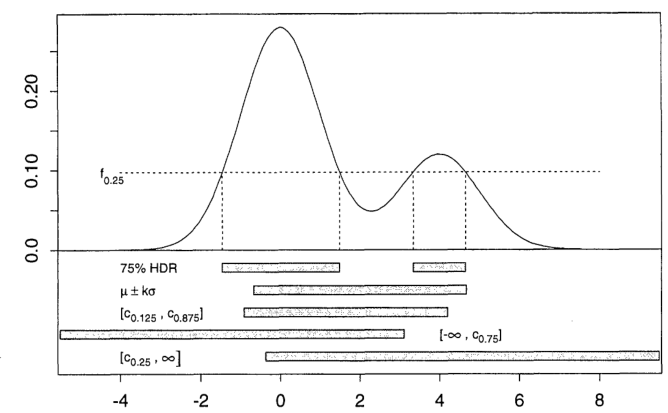
\includegraphics[width=0.9\linewidth]{figures/HPD-region.png}
    \caption{
    Illustration of a $75\%$ highest-density region for a bimodal density. The high density region (HDR, or HPD region when $f$ is a posterior density) is the density superlevel set $\{x:f(x)\geq f_{0.25}\}$, shown as two disjoint intervals. It contains the highest-density values and has the smallest total length among regions with $75\%$ probability content; the other bars show alternative connected or one-sided regions with the same probability content. Source: \url{https://stats.stackexchange.com/questions/148439/what-is-a-highest-density-region-hdr}.
    }
    \label{fig:HPD-region}
\end{figure}
